\chapter{Introduction}

Back in end of {\it 1960’s} when the Internet was a rather small 
network, which was interconnecting major universities, governmental 
and military organizations, very little attention was devoted to 
security. Nowadays, when the Internet has become extremely 
sophisticated in structure, connecting billions of devices ranging 
from small IoT type devices to humongous data-centers, security has 
gained number one priority. In present days, a typical Intranet of 
an organization can include number of geographically separated 
branch-office networks (for example, consider a factory that has 
many SCADA devices and a mission control center that is miles and 
miles away). Since these networks geographically separated, connecting 
them becomes a necessity, and so is the security of these networks. 
This is when the layer-3 virtual private networks ({\it L3-VPN}) and layer-2 
virtual private LAN services ({\it L2-VPLS}) solutions become handy. 
There are, however, other requirements that need to be taken into 
account. Scalability, resilience to various attacks, from man-in-the-middle 
to integrity violation attacks, to rather fundamental attacks on 
asymmetric algorithms (such as RSA, DSA and their elliptic curve 
counterparts, Diffie-Hellman and Eliptic Curve DH, for example) 
using, for example, {\it Shor’s quantum computer algorithm} to factorize 
large numbers, and massive brute force attacks on hash algorithms 
should be considered thoroughly. With this in mind, in this work we 
present different security solutions, which can be used to build secure 
L2 and L3 overlay networks. We present the limitations of each solution 
and identify how they can be avoided using various VPLS and L3-VPN.
We start with a background material on cryptography. 
Here we discuss various symmetric and asymmetric encryption algorithms, 
present the definition of hash functions, which considered secure nowadays, 
and discuss several key agreement algorithms. To make the discussion 
complete we present the threat that quantum computers pose for such 
algorithms as RSA and DH, and discuss how post-quantum algorithms such 
as those that are based on lattice can be used as alternative to classical 
algorithms for encryption and signature constructions. Although, not considered 
as part of the present work, future work can be include the performance 
comparison of standardized RSA and DSA algorithms with the performance of 
lattice-based algorithms incorporated into for example Host Identity Protocol 
or event Transport Layer Security protocol. We than move on to discussion of 
TLS, SSL, IPsec, HIP and SSH protocols and how those can be used to achieve 
integrity and confidentiality of data transmitted over insecure channels. 
Afterwards, we move on to the discussion of the results we have obtained 
over the course of several years. Here, we discuss our practical experience 
with scalable Host Identity Protocol based L3-VPN and VPLS network which is 
build using the same protocol. We devote a separate section on 
hardware-accelerated versions of AES and SHA-256 algorithms. We conclude 
the results section with the analysis of the limitations of each solution 
and present the results for the various micro-benchmarking settings. 


\section{Questions}

In this work, we ask several questions. These are not research questions, 
but rather practical questions we try to answer to ourselves in order to 
understand the usability of Python based security solution. Since our work 
focuses on the application of Host Identity Protocol (HIP) in VPN and VPLS 
settings we ask the following questions:

First, {\it what is the performance of the pure Python-based implementation of 
symmetric key encryption and decryption routines as well as hash methods and 
how do they compare to implementation, which uses special CPU AES and SHA-256 
instructions.} Here our focus is on the microbanchmarking of two implementations 
of AES and SHA-256 hashing algorithm, identification of the bottlenecks and 
further recommendations for our prototype implementation of Host Identity Based VPLS and L3-VPN.

Second, {\it what is the scalability of Host Identity Protocol based VPLS and how does 
it perform in emulated environments such as Mininet.} Here we seek the answer to 
the question whether the HIP-VPLS is usable in environments close to real-life setups.

Third, {\it what is the performance of Python based HIP-VPLS on real hardware}. By 
doing so we want to find the application niche of our security solution. In addition, 
we discuss the practical configuration of HIP-VPLS using central controller.

The next question {\it we want to answer relates to the deployment of scalable L3-VPN 
based on Host Identity Protocol}. Here we focus on rather different approach of building 
secure networks: We consider L3-VPN where nodes in different branches offices form separate 
broadcast domains, but still can communicate with each other (with assistance of IPv4 
routing protocol). Here, we want to answer how to tackle the scalability issues of 
VPN network by adding hierarchy into the architecture.


\chapter{Background}

Since we are going to discuss the security protocols in this work, we begin 
this section with the shallow dive into cryptography basics. Here, we discuss 
symmetric and asymmetric cryptography algorithms, to make the description a 
little bit complete we show how RSA algorithm works, discuss the math behind 
Diffie-Hellman (DH) and its Elliptic Curve counterpart. We will also discuss 
the Shor’s algorithm and its quantum computer implementation that theoretically 
can efficiently factorize big number. This algorithm, if powerful enough quantum 
computers will exist in the near future, puts the RSA algorithm - the major 
building block of modern security solutions - at risk of being cracked (once the 
modulus of RSA algorithm factorized into prime components, the private key of RSA 
algorithm can be easily recovered). We will conclude this part of the background 
material with the discussion of post-quantum computer public key encryption 
solution based on lattice (more specifically we will discuss Learning With Errors 
(LWE) algorithm). We believe that, eventually, this type of cryptography will be 
the replacement for traditional RSA and DH algorithms, which rely on the hardness 
of factorization of the big numbers and discrete logarithms. In the epilogue of this 
section, we will put few words on how lattice public key cryptography can be used, 
for example, together with Host Identity Protocol.

In the second part of the background material, we will review the basics of the Host 
Identity Protocol, Transport Layer Security Protocol and Secure Shell Protocol, since 
these protocols are the main building blocks of secure tunneling protocols that we
discuss in this work.

We will finalize the discussion of the background material with a short overview of 
various L2, L3 and L4 tunneling solutions, including L2 802.1Q QinQ tunneling, 
L3 Multi-Protocol Label Switching (MPLS) VPLS, L4 TLS and SSH tunneling.


\section{Cryptography basics}

Cryptography comes in many flavors: symmetric key cryptography 
(3DES, AES, Twofish, RC4) which, in turn, can be categorized into 
block cipher and stream cipher and asymmetric key cryptography 
(such as RSA, DSA, ECDSA). There are also key exchange protocols 
such as Diffie-Hellamn and Elyptic Cryptography DH for negotiation 
of common keys over insecure channels. Different algorithms applicable 
in different settings depending on requirements. Typically, as we will 
discuss later, symmetric key cryptography is used to protect 
data-plane traffic in networks, whereas, asymmetric-key cryptography is 
more applicable to the common key negotiation, authentication and 
identification purposes~\cite{Stinson:Cryptography}.

\subsection{Symmetric cryptography}

We start with the symmetric key cryptography. Common key and rather 
trivial operations such as permutations and substitutions are at the 
heart of any symmetric key cryptography algorithm. Although, this type 
of cryptography is efficient because of the usage efficient operations, 
it comes with a limitation though. In symmetric key cryptography, 
both sender and receiver need to share the same key, which complicates 
such important aspects as key distribution and revocation and so alone 
this encryption solutions a very hard to use alone in modern cryptosystems. 
Typically, asymmetric key cryptography such as RSA used to derive session 
keys – TLS, HIP and many other protocols follow this design idea.

Symmetric key cryptography comes in two different flavors: block and stream. 
For example, block cipher (such as AES, 3DES, Twofish~\cite{Stinson:Cryptography}) 
use blocks of data (typically, the size of the block is 128, 160, 256 
bits~\cite{Stinson:Cryptography}), and encrypts or 
decrypts one block at a time. There are different modes of operation, though, 
for block ciphers, examples are counter mode and cipher block chaining. The latter 
one uses so-called initialization vector to add extra randomness into encryption 
process, and encryption of proceeding blocks depends on the output of the previous 
block. Modes of operations are important for security reasons. However, not all 
modes of operations useful and secure. For example, Electronic Code Book (ECB), 
while allow achieving fast processing and parallelization, is considered insecure in 
many settings. In Figure[] we demonstrate AES encryption in CBC mode:

The other type of symmetric key algorithms is stream cipher. Here the encryption 
and decryption performed on separate bits, one bit at a time. CR4 is an example 
of stream cipher. Stream ciphers are extremely important in real-time processing, 
for example, Wi-Fi uses stream ciphers to encrypt the data plane traffic.

\subsection{Asymmetric cryptography}

Asymmetric key cryptography, in its simplest form, is the brilliant in the age 
of computing. Guessing from the name that this type of cryptography uses different 
keys for encryption and decryption does not require deep though. This property makes 
this group of algorithms suitable for various key distribution, revocation and 
signature ideas. 

There is a magnitude of different asymmetric key security algorithms. 
RSA, DSA and its Elliptic curve variant ECDSA are the pillars of modern 
security solutions. But the flexibility of these schemes comes at an extra 
price of CPU cycles. All this makes these solutions inapplicable for securing 
data plane traffic, but only rather to secure control plane. In what follows, 
just to underpin the beauty of the math behind asymmetric key cryptography, 
we provide a description of RSA algorithm.

In RSA cryptosystem, the sender generates a pair of keys as follows: 
First, the sender chooses large enough two prime numbers $p$ and $q$. Next, 
the sender computes $n=pq$ and evaluates Euler’s phi function: $\phi(n)=(p-1)(q-1)$. 
This is the same as the number of numbers co-prime to $n$. The sender then selects at 
random encryption exponent $e$ such that $1<e<\phi(n)$ such that $e$ is co-prime to $\phi(n)$ 
and computes the decryption exponent d such that $ed \equiv 1\ mod\ \phi(n)$ using modular 
multiplicative inverse.

The public key is then $(n, e)$ and the private key is $(n, d)$. To encrypt the message $m$ 
the sender computes $c= m^e\ mod\ n$. The decryption is similar $m = c^d\ mod\ n$. The beauty is 
in Fermat’s little theorem, which states that $m^{\phi(n)}\ mod\ n \equiv 1\ mod\ n$. 
Now, $ed\ \equiv\ 1\ mod\ \phi(n)$, which means that 
$ed=k\phi(n)+1$, and so $m^{(ed)}\ mod\ n \equiv m^{(k\phi(n)+1)} mod\ n \equiv 1^k m\ mod\ n \equiv m\ mod\ n$. 

In practice, RSA requires random padding to protect against such attacks as chosen ciphertext 
attacks and making two identical plaintext produce various ciphertexts. Padding also ensures that the 
message size is multiple of encryption block-size. In practice, Optimal Asymmetric Encryption Padding (OAEP) 
scheme is used [].

It is good to know that if the message hashed and encrypted with private key, the result is a 
form of digital signature, since the sender cannot later deny that it was involved into encryption 
process. Digital Signature Algorithm (DSA) is another example of asymmetric signature scheme and 
was specifically design for that purpose. Elliptic Curves another version of DSA algorithm.

Frankly speaking, symmetric signature schemes can be also used. For example, one can use 
one-time hash-based signatures to produce the secure digital signatures. Nevertheless, 
the application of these type of signature algorithms is rather impractical and finds 
little application in real-life settings.

\subsection{Cryptographic hash functions}

Mathematically, speaking hash function is special function that given a 
pre-image of an arbitrary size produces an image or hash of a fixed size, 
which is universally unique. Secure hash functions guarantee, to a certain 
degree, that the result of a hash function is irreversible. That it is, it 
should be extremely hard to find a pre-image, or original message, given a 
hash or fingerprint. Secure hash functions should be also collision resistant. 
In other words, it should be extremely hard, if not impossible at all, to 
find two different messages $m$ and $m’$ that will hash to the same value, i.e., 
$hash(m)=hash(m’)$.

Secure hash functions are important in modern cryptography. 
For example, they serve as authentication tokens for transmitted message over the 
wire (useful, for example, in detecting message manipulation during transmission), 
they allow compressing the message before signing it with the digital signature 
algorithm, and they can be used to find the differences between the messages 
efficiently. The application area is of course broader than just these few examples. 

Hash functions come in different flavors, but good ones should be computationally 
efficient and resistant to collisions. Today, hash functions such as MD2, MD4 and MD5 
considered broken, as there are works that showed successful attacks. Briefly speaking, 
researchers successfully found collisions for this hash functions. Therefore, it is 
not recommended to use these hash functions in security applications. A more modern 
family of SHA hash functions also exists. For example, engineers recommend using SHA-256, 
SHA-512 and SHA-3 in modern applications, as no successful attacks were registered for 
these types of hash functions.

Hash functions pave a road for such a notion as authentication tokens when combined with a 
secret key in a special way. Examples are HMAC [], PMAC, CMAC which is based on AES cipher. 
For instance, by sending an HMAC together with the original message one can make sure that 
the message will not be tampered during the transmission. In addition, if the message will 
be altered on the path to recipient, this fact will be flagged immediately during the 
verification process.

Hash functions are also useful in signatures. For example, one-time signature are using 
hash functions to construct an digital signature of a message. An interested reader can 
find more information about hash functions here [].

\subsection{Key exchange protocols}

Key exchange are important in modern systems as they allow negotiation of common 
key over insecure channel. Of course, RSA can be used to deliver a session key
by encrypting it with the recipients public key, but specially crafted key negotiation
algorithms exist in practice. Two bright examples are Diffie-Hellman (DH) and Eliptic Curve 
DH. 


\subsection{Post-quantum Lattice-based cryptography}

Shor's algorithm, implemented on quantum computer makes certain computational 
problems (such as, factoring of large numbers and discrete logarithm problem) 
feasible in polynomial time. This shutters the security of the Internet, and 
so rigorous research was initiated to fill the gap. In what follows we discuss
certain hard mathematical problem on lattices and show the workings of the 
Learning With Errors (LWE) public key encryption scheme. In fact majority of 
NIST's candidates for post-quantum public key encryption algorithms are based 
on LWE.

A lattice is a mathematical structure which consists of integers in $n$-dimensions 
arranged in a structured lattice-like way. Mathematically, the lattice is defined as follows:
$$\Lambda({\bf B}) = \{{\bf Bx}, {\bf x} \in \mathbb{Z}^n \}$$ where ${\bf B}$ is a matrix of basis vectors
that generate the lattice. We should note that there exist large number of basis vectors, some are {\it good}
some are {\it bad}.

A { \bf closest vector problem (CVP) } on lattices, which is considered NP-hard, is not solvable even on 
quantum computers, can be defined as follows. Given a point $t \in \mathbb{R}^n$ and a lattice
$\Lambda({\bf B})$, the task is to find a closes point ${\bf Bx}$ on lattice: 

$$\min_{\forall {\bf x} \in \mathbb{Z}^n} \|{\bf Bx} - {\bf t}\|$$ 

In practice the above problem is extremely hard to solve which makes lattice-based cryptography 
attractive to cryptographers.

From linear algebra we know that solving equation $\bf{Ax}=\bf{b}$ is simple using
Gaussian elimination. However, if a random noise is added to the equation $$\bf{Ax} + \bf{e} = \bf{b}$$ the 
problem is considered as hard as CVP on lattice. Solving the above problem directly relates to 
solving the CVP problem on lattice if the parameters are selected carefully.

Given a matrix $\bf{A} \sim U(\mathbb{Z}^{nxm}_q)$, $\bf{s} \sim U(\mathbb{Z}^{n}_q)$ and $\bf{e} \sim D_{\mathbb{Z}^{m}, \sigma}$ 
sampled from discrete (clipped) Gaussian distribution with parameter $\sigma$. We require that, the probability
$P[e < q/4]$ is high (\ie $99.99\%$) to ensure correct decryption of the message and to achieve required 
level of security. This can be achieved by setting the parameter for discrete normal distribution carefully, \ie $4\sigma < q/(4m)$.

To ensure that $\bf{re}$ is always less than $q/4$ the values are drawn with resampling
or clipping. We require, further, that the parameter $\sigma = q/(16m)$. We now defined 
matrix ${\bf A}$, secret key ${\bf s}$ and noise vector ${\bf e}$ as follows:

\begin{equation}
    {\bf A}=\begin{bmatrix}
        a_{11}       & a_{12} & a_{13} & \dots & a_{1n} \\
        a_{21}       & a_{22} & a_{23} & \dots & a_{2n} \\
        \hdotsfor{5} \\
        a_{m1}       & a_{m2} & a_{m3} & \dots & a_{mn}
    \end{bmatrix}
\end{equation}

\begin{equation}
    {\bf s}=\begin{bmatrix}
        s_{1} \\
        s_{2} \\
        \dots \\
        s_{n} 
    \end{bmatrix}
\end{equation}

\begin{equation}
    {\bf e}=\begin{bmatrix}
        e_{1} \\
        e_{2} \\
        \dots \\
        e_{m} 
    \end{bmatrix}
\end{equation}

Once the parameters are generated, we can compute ${\bf As}+{\bf e} = {\bf b}$. Then, the public 
key is $({\bf A, b})$ and the private key is ${\bf s}$. Deriving ${\bf s}$ from ${\bf b}$ is a hard 
task at hand.

To encrypt the message $\mu \in \{0, 1\}$ choose ${\bf r} \sim U(\{0, 1\}^m)$. Then compute ${\bf u}={\bf rA}$ and 
$v={\bf rb}+\lfloor q/2 \rceil \mu$. The ciphertext is $({\bf u}, v)$. To decrypt the message 
compute $v - \bf{u s}$, if the result is less than $q/4$ output $0$, if the result
is larger than $q/4$ output $1$. 

The major disadvantage of lattice-based cryptography is the size of the keys and actual ciphertext. For example,
security of LWE depends on two parameters $n$ and $q$. By choosing $n=512$ and $q=2^{16}$, the size of ciphertext
for a message of $k=256$ bits long (for example, this is the size of the key for AES-256 symmetric algorithm), 
the size of the ciphertext will be $O(k \cdot n \cdot \log q) \approx 256 \cdot 16 \cdot 512$ bits or roughly whooping 
$256$ KB. All in all the security does not come for free. Of course, there are way much practical implementations
if LWE-based encryption algorithms, for example, the reader can take a look at Kyber~\cite{nist:kyber} which has practical 
implementation in TLS library.

\section{Security protocols}

Equipped with basic understanding of the cryptography we will now dive into discussion of some 
of the well-known security protocols, including IPSec, HIP, TLS and SSH. All these protocols
make a solid basis for the secure internetworking.

\subsection{Host Identity Protocol (HIP)}

Internet was designed initially so that the Internet Protocol (IP) address has a dual role: it 
is the locator, so that the routers can find the recipient of a message, and it is an identifier 
so that the upper layer protocols (such as TCP and UDP) can make bindings (for example, transport 
layer sockets use IP addresses and ports to make connections). This becomes a problem when a networked 
device roams from one network to another, and so the IP address changes, leading to failures in 
upper-layer connections. The other problem is the establishment of an authenticated channel between 
the communicating parties. In practice, when making connections, the long-term identities of the parties 
are not verified. Of course, solutions such as SSL can readily solve the problem at hand. However, SSL 
is suitable only for TCP connections, and most of the time, practical use cases include only secure web 
surfing and the establishment of VPN tunnels. Host Identity Protocol, on the other hand, is more flexible: 
it allows peers to create authenticated secure channels on the network layer, so all upper-layer protocols 
can benefit from such channels. More on the protocol can be found in~\cite{gurtov:hip}.

HIP relies on the 4-way handshake to establish an authenticated session. During the handshake, the 
peers authenticate each other using long-term public keys and derive session keys using Diffie-Hellman 
or Elliptic Curve (EC) Diffie-Hellman algorithms. To combat the denial-of-service attacks, HIP also 
introduces computational puzzles. 

HIP uses a truncated hash of the public key as an identifier in the form of an IPv6 address and 
exposes this identifier to the upper layer protocols so that applications can make regular 
connections (for example, applications can open regular TCP or UDP socket connections). At the 
same time, HIP uses regular IP addresses (both IPv4 and IPv6 are supported) for routing purposes. 
Thus, when the attachment of a host changes (and so does the IP address used for routing purposes), 
the identifier, which is exposed to the applications, stays the same. HIP uses a particular 
signaling routine to notify the corresponding peer about the locator change. More information 
about HIP can be found in RFC 7401. 

\subsection{Secure socket layer (SSL)}
Secure socket layer (SSL)~\cite{ssl} and Transport Layer Security (TLS) are an application 
layer solutions to secure TCP connections. SSL was standardized in RFC 6101. 
TLS was standardized in RFC 5246. And was designed to prevent eavesdropping, man 
in-the-middle attacks, tampering and message forgery. In SSL the communicating 
hosts can authenticate each other with help of longer term identities - public key certificates.
SSL is great for building VPN tunnels and protecting upper layer protocols such as HTTP


\subsection{Secure Shell Protocol (SSH)}

Secure Shell protocol (SSH) is the application layer protocol which provides an encrypted channel 
for insecure networks. SSH was originally designed to provide secure remote command-line, login, 
and command execution. But in fact, any network service can be secured with SSH. Moreover, SSH 
provides means for creating VPN tunnels between the spatially separated networks: SSH is a great 
protocol for forwarding local traffic through remote servers. 

\section{L2, L3 and L4 tunneling}

Virtual Private LAN Services (or VPLS), L3-VPNs, L4 tunneling are pretty standard nowadays. 
Companies build security solutions to provide Layer-2 and Layer-3 services for branch offices: 
VPLS are typically built as overlays on top of Layer-3 (IP) and are Ethernet over IP type 
overlays, whereas L3-VPNS are IP-in-IP tunneling solutions.

In VPLS, when a frame arrives at VPLS provider equipment (PE), it is encapsulated 
into an IP packet and is sent out to all other VPLS network elements comprising emulated LAN. 
Security of such overlays is important for obvious reasons: customers do not want their corporate 
traffic to be sniffed and analyzed. In L3-VPN networks, on the other hand, the networks form different 
broadcast domains, and so when IPv4 or IPv6 packet arrives at VPN box, it is encapsulated into another 
IP packet and sent out using the backbone network. In this work, we built such secure overlays with 
Host Identity Protocol. 

In this section, however, we will briefly review some of widely existing solutions 
for building L2, L3 and L4 overlays.

\subsection{Virtual Private LAN Services (VPLS) L2VPN solutions}

Virtual Private LAN Services (VPLS) are pretty common nowadays. In this section we will cover 
to standard ways to build VPLS networks (802.1 QinQ tunneling and MPLS).

\subsubsection{QinQ tunneling}

When the path from one network to the other, such as branch office to head office,
traverses only layer-2 switches (\ie no IP routing is involved), the VPLS can be organized 
with the help of 802.1Q protocol~\cite{snr}. Broadly, speaking this is not a protocol as such, but rather 
VLAN tag based switching. Thus, on ingress point an additional 802.1q service provider SP-VLAN tag 
is inserted in L2 header of an Ethernet frame. Later, the forwarding decisions are 
made using this SP-VLAN tag. On egress point the SP-VLAN tag is removed and original 
Ethernet frame is forwarded to the recipient based on destination MAC address 
and, if exists, on inner C-VLAN tag. 

It should be noted that the configuration of forwarding is a manual configuration step.
Also, QinQ does not provide additional mechanisms to secure the customer's traffic,
thus limiting the application domain of this solution.

\subsubsection{MPLS tunneling}

Multi-protocol label switching is a standard protocol for forwarding any traffic type.
It has label distribution protocol and label switching components. It is an ideal way 
of forwarding the traffic even if path contains L3 routers.

\subsection{Virtual Private LAN (L3-VPN) security solutions}

The major drawback of QinQ and MPLS and QinQ is that they do not offer encryption and 
authentication of traffic. Therefore, additional steps needs to be taken to protect end-to-end
traffic. In this section we will review PPTP, SSL-based VPNs, L2TP and IPsec tunnels.

\subsubsection{Multipoint to single point VPN}

Multipoint to single head VPN is a standard way of organizing VPN network
for an organization that has single head office and multiple branch offices.
In this setup multiple branch offices are connected to a head end. 
We show such setup in Figure~\ref{fig:head-vpn}.

\begin{figure}[ht!]
    \centering
    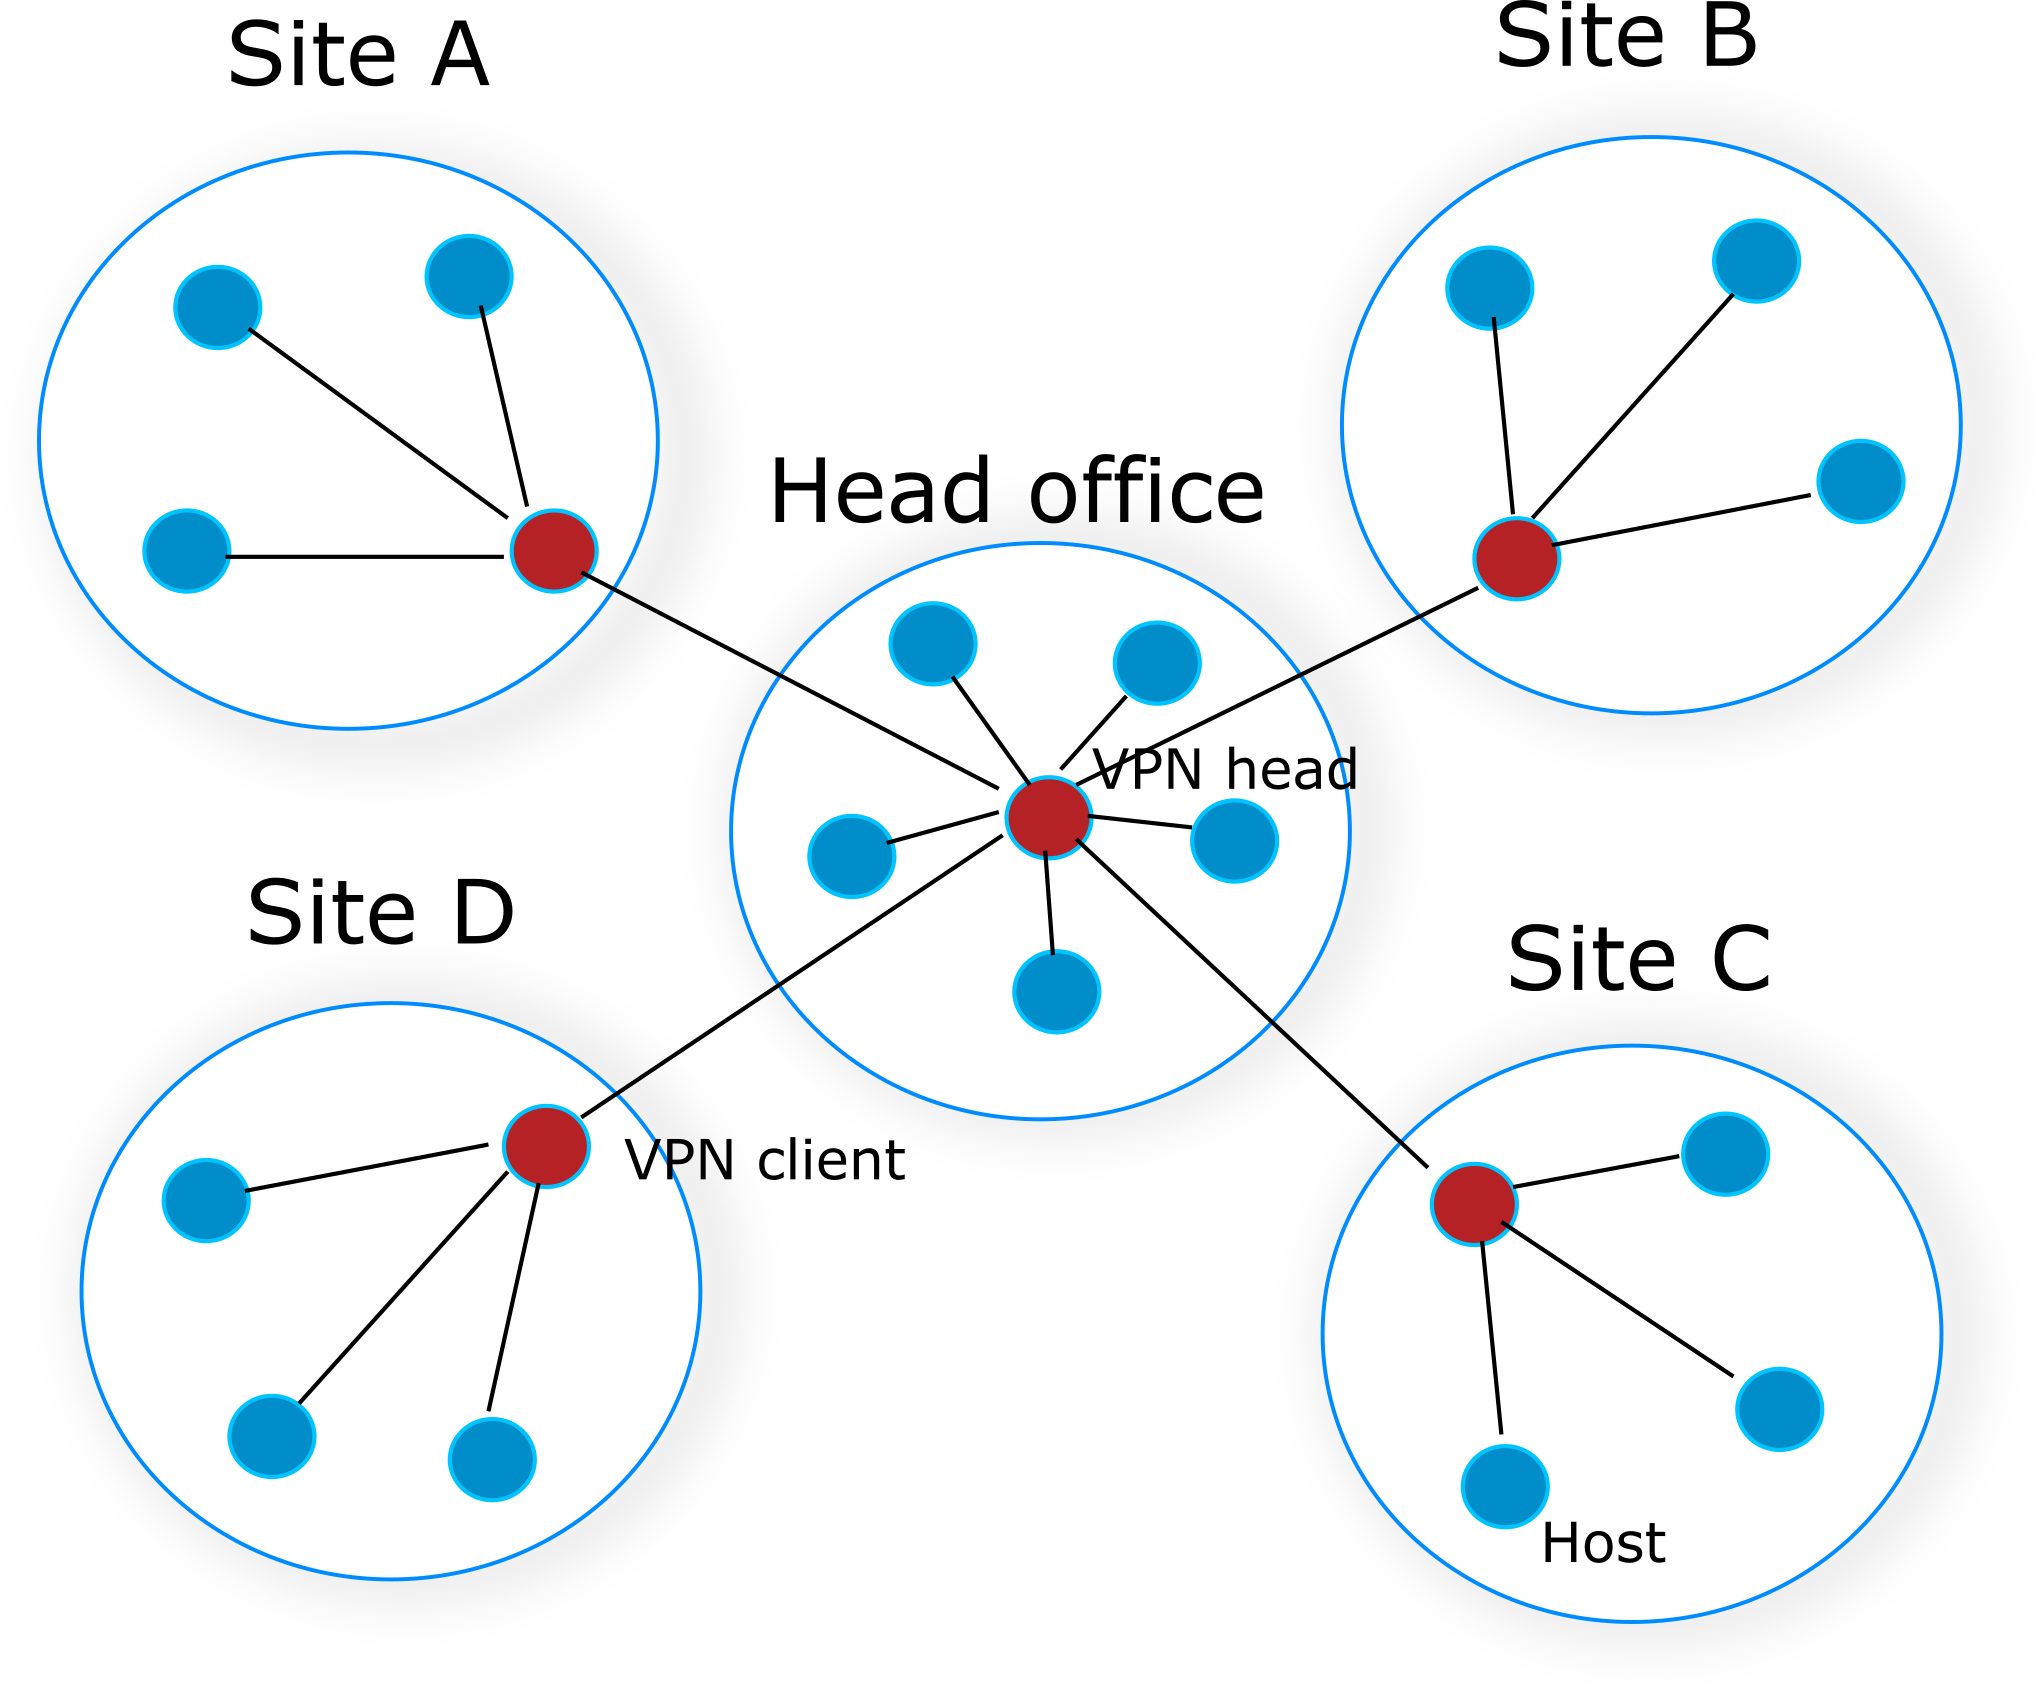
\includegraphics[width=0.9\textwidth]{graphics/vpn-central.png}
    \caption{Typical arrangement of the VPN}
    \label{fig:head-vpn}
\end{figure}

There is a number of protocols available for such an arrangement. Examples are:
(i) Point-to-Point Tunneling Protocol (PPTP); (ii) SSL-based 
Secure Socket Tunneling Protocol (SSTP); (iii) Layer 2 Tunneling Protocol (L2TP), 
which is an older protocol that can be combined with IPSec for encryption; 
(iv) Internet Protocol Security (IPSec). 

We have, ourselves, created one particular implementation that is based on SSL~\cite{ssl:vpn}.
The idea is to tunnel all traffic from VPN agnostic hosts through a off-the-path 
black box that encrypts all the traffic and sends encapsulated in TCP and SSL
to the L3-VPN head server. The solution that we have created is a simple script 
that allows to setup such an arrangement with no hassle. One drawback is that it 
uses TCP for transport: sending over reliable TCP channel and over well known HTTPS port
is good for bypassing the traffic filters, but reduces the performance especially if
the channel has large latency and error rate. 


\subsubsection{SSH tunneling}

SSH, despite that it was invented for remote access to Linux-like boxes, can be used 
to tunnel local to remote and remote to local traffic~\cite{ssh:tunneling}. Thus it can be used to create
layer-4 tunnels. For example, the following command will tunnel all local traffic from
port 4443 to remote web-server {\it youtube.com} on port 443:

\begin{verbatim}
ssh -L 192.168.1.1:4443:youtube.com:443 user@strangebit.io
\end{verbatim}

In this example, when the client types \url{https://192.168.1.1:4443/} in the browser window,
the traffic will be forwarded to the remove youtube server through the SSH server \url{strangebit.io}.

There is also a possibility to perform the reverse tunneling, \ie one can expose the local service to the world.
For example, suppose you have a precious MySQL resource in your local network running on host \url{192.168.1.45} 
on port $3306$, then you can expose the service to the world using the following command:

\begin{verbatim}
ssh -R 0.0.0.0:3306:192.168.1.45:3306 user@strangebit.io
\end{verbatim}

This way various tunneling setups can be organized making SSH an attractive secure tunneling 
solution.

\chapter{Results}

In this chapter we are going to present the results that we have obtained 
throughout several years that we have spent building various systems. We start 
with the results for cryptographic library which we have implemented to 
boost the performance of AES and HMAC algorithms on Intel CPUs. We then 
present the results for complete HIP-VPLS architecture and present the 
looking of the web interface which was used to configure the HIP switches.
Finally, we present the design and implementation of the hierarchical L3-VPN
in Mininet emulator.  

\section{Hardware-enabled symmetric cryptography}

Part of the work that we have done was related to porting parts of the code to pure C 
and special Intel CPU instructions. In this section we will describe our achievements 
in this direction. 

For the benchmarkings we have selected three implementations. The first one was pure 
Python based. For that purpose we have used PyCryptodome library. The second implementation
was a Python wrapper to C library that was using special Intel CPU instructions to boost 
the AES and SHA-based HMAC operations. The third implementation was pure C library 
which was using Intel NI instructions. The results for AES-256 and HMAC operations 
for varying block sizes is shown in Figure~\ref{}. The plots show the average 
running time in microseconds with the $95\%$ confidence intervals. 

\begin{figure}[h!]
    \centering
    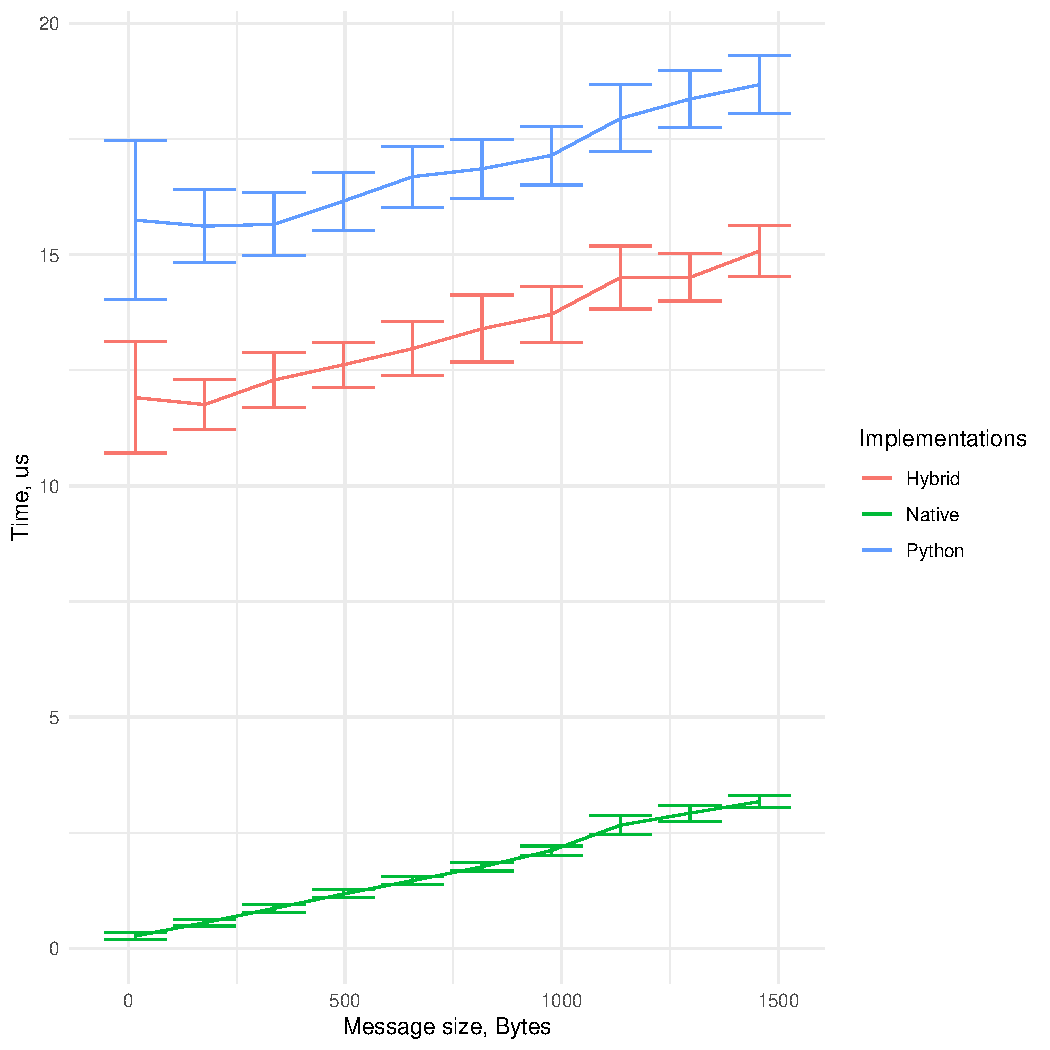
\includegraphics[width=0.9\textwidth]{graphics/crypto/aes.pdf}
    \caption{AES-256 encryption (microseconds)}
    \label{fig:aes}
\end{figure}

\begin{figure}[h!]
    \centering
    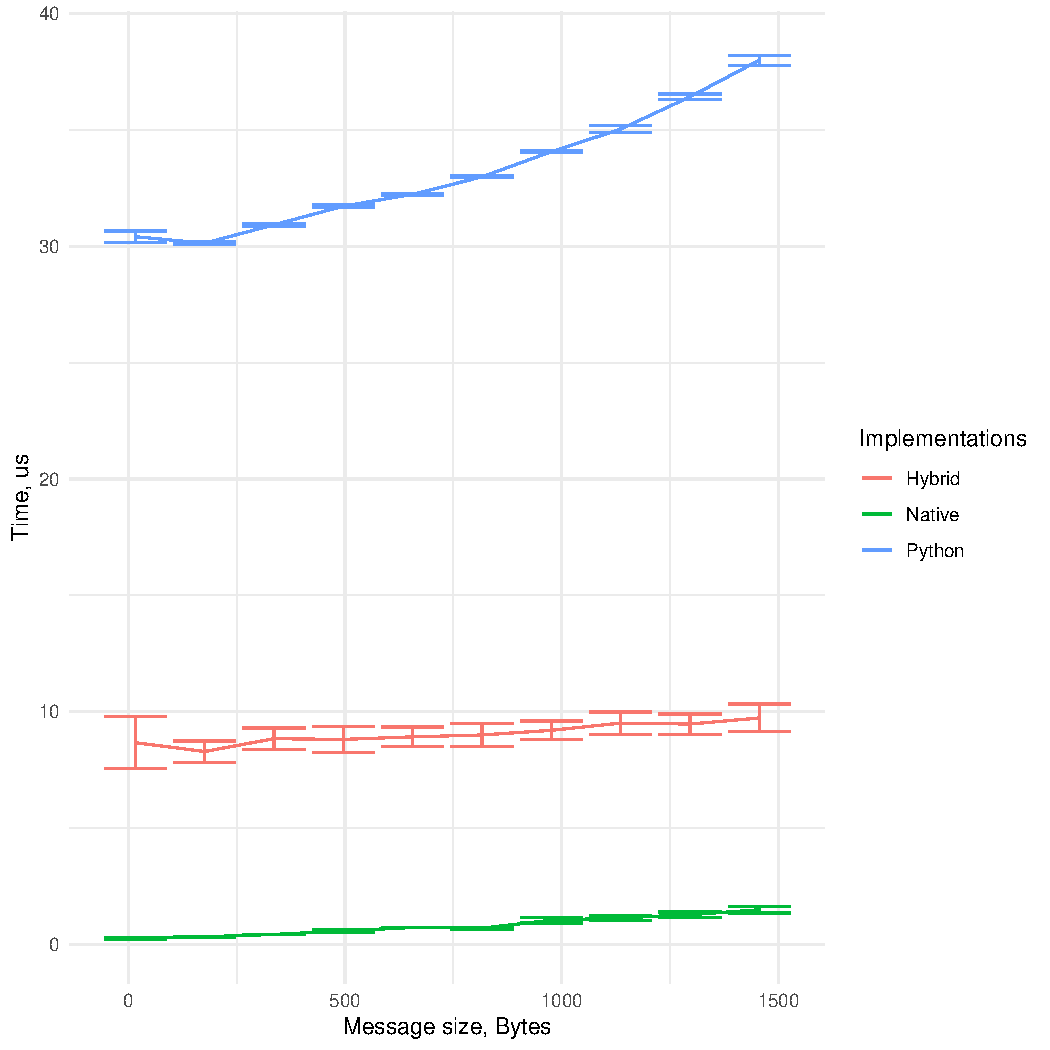
\includegraphics[width=0.9\textwidth]{graphics/crypto/hmac.pdf}
    \caption{HMAC calculation (microseconds)}
    \label{fig:aes}
\end{figure}


What related to cryptographical operations. For standard packet of size $1500$ 
bytes we have compared the performance (combined HMAC and AES-256) and it turned 
out, on one hand, that implementation of cryptography in pure C with CPU instructions is 
$12.1$ faster than pure Python implementation. On the other hand, Python implementation with bindings
to C library demonstrated performance which was $2.3$ times faster. By making back of the envelop calculations
we predict that Python implementation can achieve roughly $461$ Mbits/s in upload and download directions
cumulatively. However, in practice, given other operations with packets we did not get this result 
in our experiments (more about performance of HIP-VPLS on real hardware can be found in proceeding 
chapter). For the plain C implementation with AES and SHA instructions the performance would be 
better and constitute astonishing $2.5$ Gbits/s. Would someone need to run the code in production
the entire code needs to be rewritten in plain C programming language.

\section{Host Identity Protocol based VPLS}

Virtual Private LAN Services (VPLS) provide means for building Layer 2 communication 
on top of existing IP networks. VPLS can be built using various approaches. However, 
when building a production-grade VPLS solution one needs to have a clear picture of 
how such aspects as security, mobility, and L2 issues will be solved.

In what follows, we will demonstrate how to build the VPLS using Host Identity Protocol (HIP). 
Our initial goal was not to build a production-grade implementation of HIP-switches. Instead, 
at first we were only interested in demonstrating proof of a concept solution that uses 
Mininet – a framework for emulating L2 and L3 networks. It is worth mentioning that the code 
we have produced can be also deployed (under certain conditions; for example, our HIP implementation 
does not feature the NAT traversal mechanisms) on the real hardware. And we are going to demonstrate 
working prototype in the later part of this document. Our prototype uses Python-based HIP~\cite{pyhip} 
as the bases for prototype.

While building HIP-switches (the switches that are deployed at the border of a network) 
we came across several challenges. First, to avoid loops the underlying network needs to support 
the IEEE 802.1D protocol (or its modification - this really depends on the version of the protocol 
supported by the switches). This problem was initially addressed in the relevant IETF draft. 
Second, there were certain issues with MTU and the inability of the Linux kernel to deliver IP 
packets when those are fragmented in user space and injected into the network stack using raw 
sockets. And finally, it took us some time to repackage the existing implementation of HIP protocol 
as a library, so that it will be agnostic about low-level networking (such as raw sockets, etc.). 
In proceeding paragraphs, we will demonstrate the usage of HIP-based VPLS using loop-free L2 topology,
that is achieved by using 802.1d STP protocol.

The working prototype logical network diagram is shown in the Figure~\ref{fig:mininet}.

\begin{figure}[h!]
    \centering
    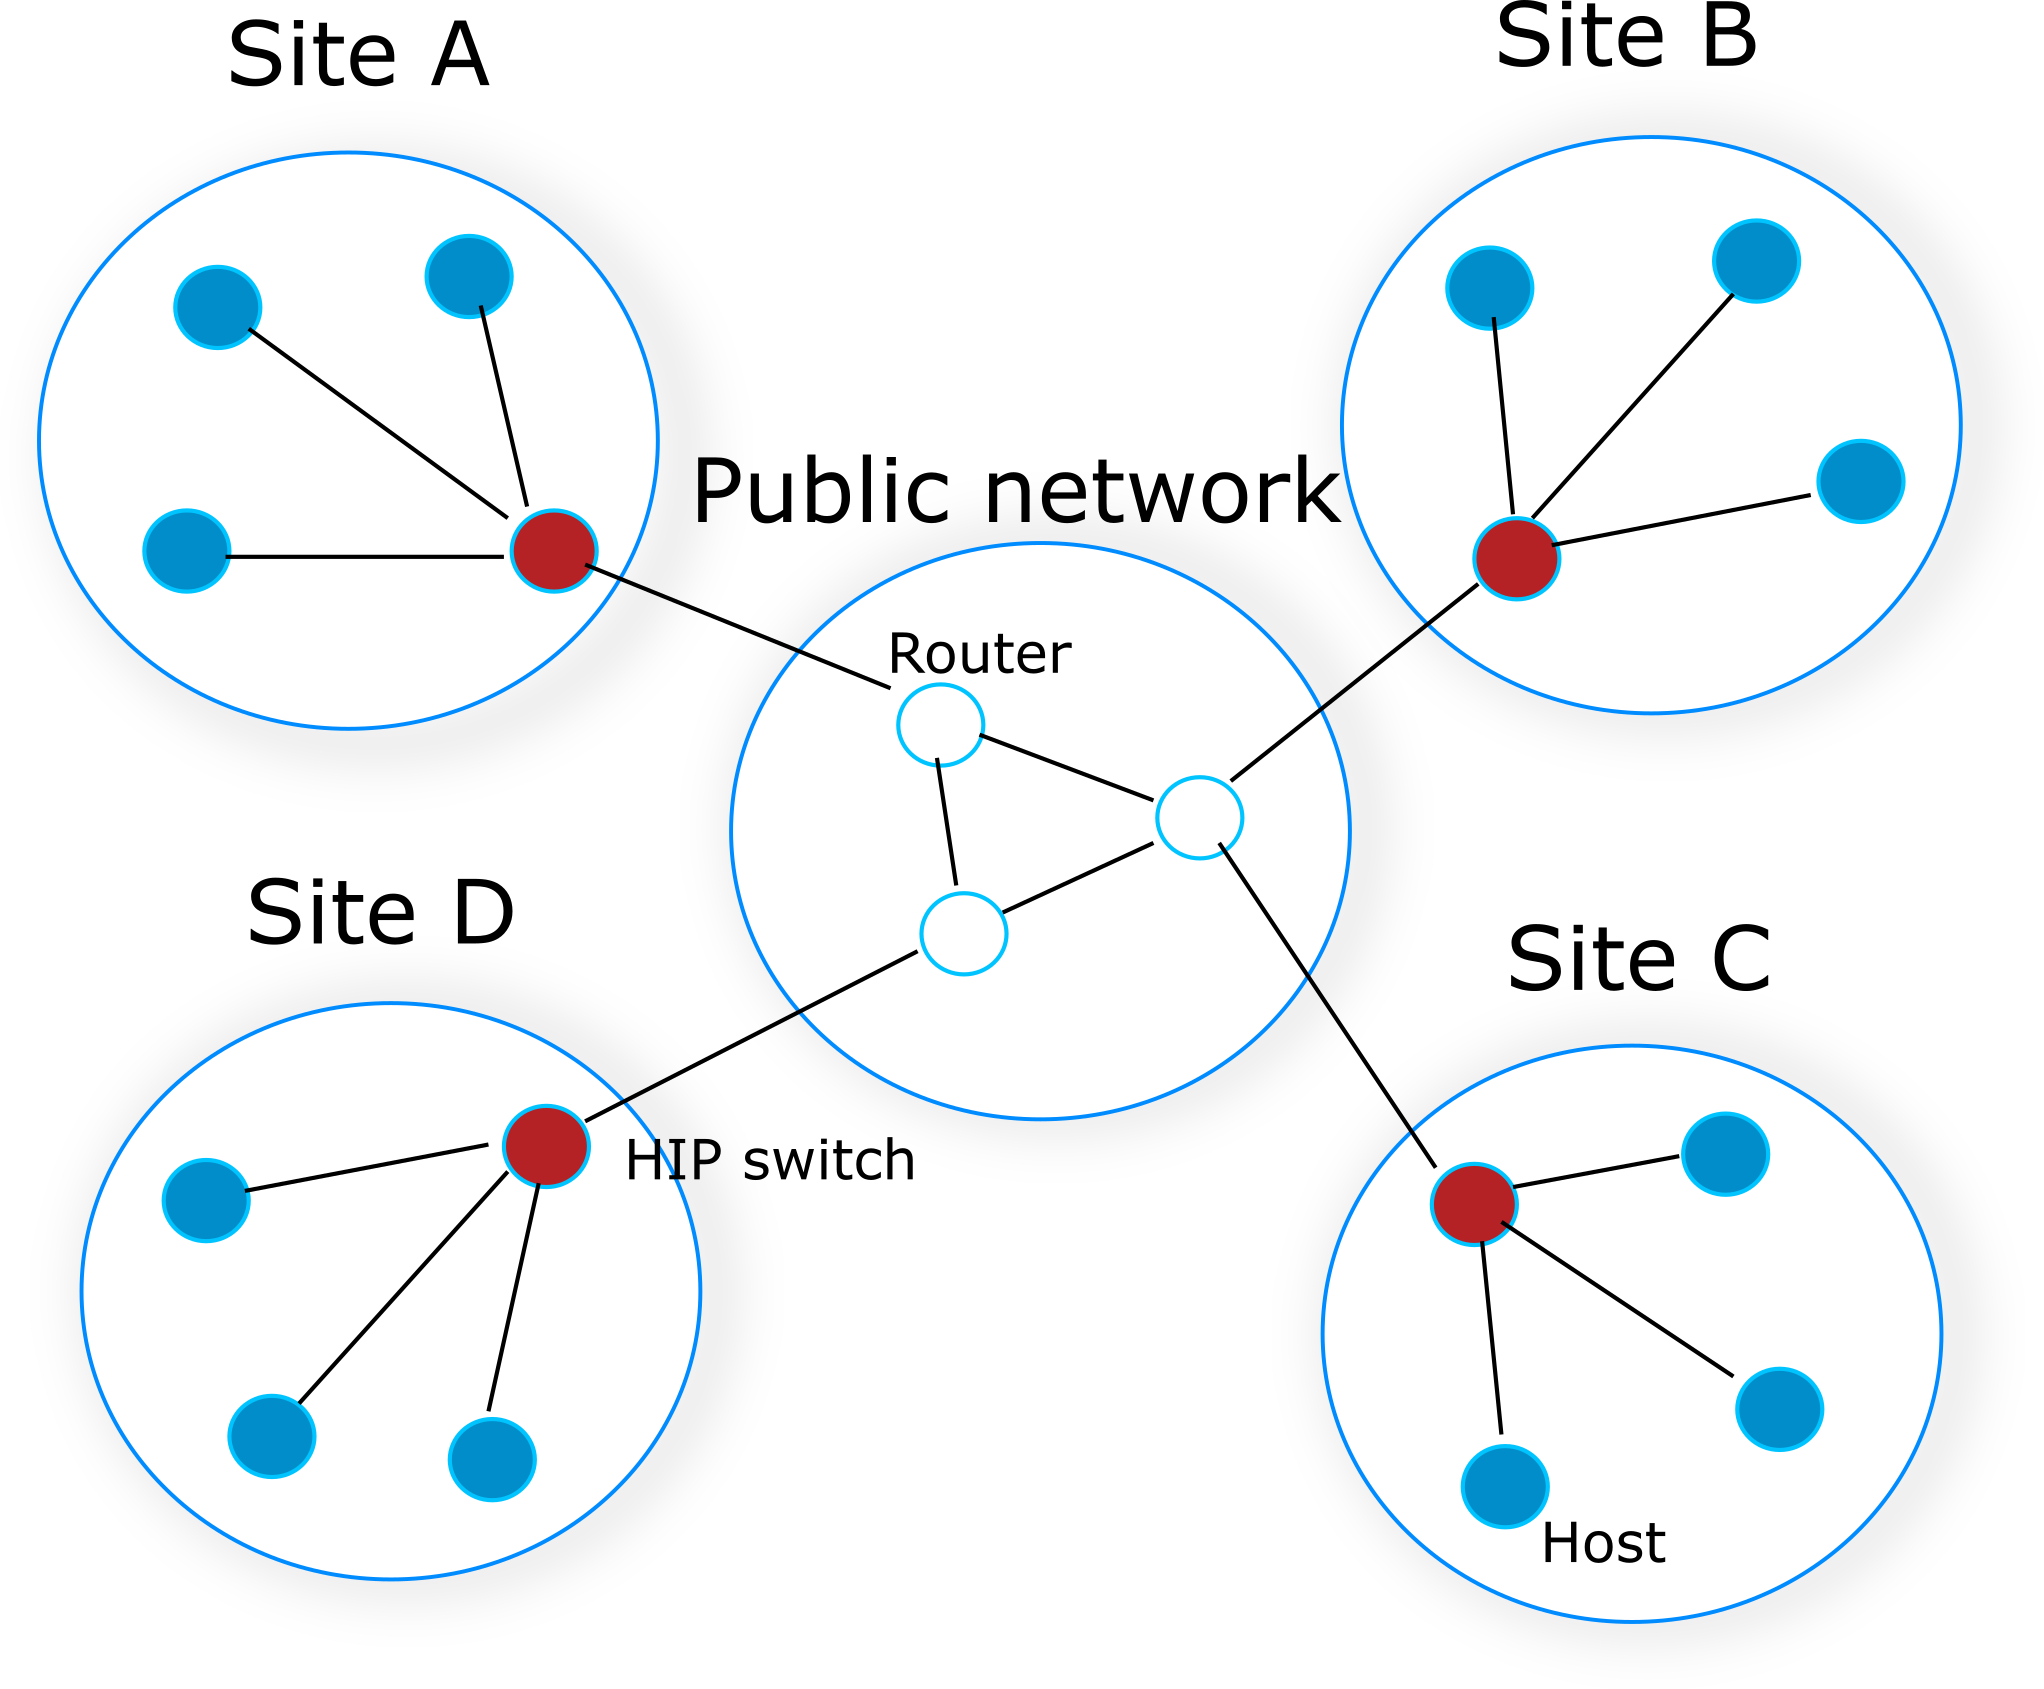
\includegraphics[width=0.7\textwidth]{graphics/mininet.png}
    \caption{Mininet HIP-VPLS logical diagram}
    \label{fig:mininet}
\end{figure}

We now turn our attention to our attention to real-life deployment 
of HIP-VPLS. The system architecture is shown in Figure~\ref{fig:architecture}. 
Apart from the HIP-VPLS switches, we have also implemented a unique 
control-plane protocol on top of the SSL protocol. 

In our deployment we have used the following setup. For HIP switches we 
have used the dual-network Intel N95 computing platform. We have used $8$ 
port SNR switches to connect 3 HIP switches, that way we have mimicked the 
IP overlay in the setup. HIP switches had two interfaces: one is facing 
LAN network, the other one is facing the WAN network. The microcomputers for
HIP switches had the following characteristics: they had $1$GB of RAM memory, 
dual core Intel N95 CPU (with support for AES and SHA2 NI instructions), 256 of 
solid state hard drive. To wire the routers we have used SNR switches 
(each switch had $8$ $1$ Gbit/s ports, and two Small Form Factor (SFP) slots). 
The testbed configuration is shown on the Figure~\ref{fig:testbed}

%In our architecture, HIP switch controller is a central server instance that collects information from the HIP-switches
%and allows one to perform configuration of such parameters as firewall rules, HIP hosts file, MAC-based access
%controll lists (ACL) and configure traffic shaper. We are going to discuss each feature seperately 
%in the proceeding paragraphs.  


According to the protocol, on the one hand, every HIP-VPLS 
switch reports to the central controller (and is authenticated 
using the HMAC algorithm together with the shared symmetric 
master secret). In the implementation switches report their presence every $5$ 
seconds. On the other hand, every HIP-VPLS switch obtains 
the configuration from the central controller (such as mesh 
configuration, HIT resolver information, firewall rules, and 
MAC-based ACL). The architecture of HIP-VPLS switches is such
that extra functionality can be easily implemented. For example,
such thing as traffic shaper can be incorporated into the design
quite easily. For example, HIP-switch, when configured centrally, 
can be serve different traffic flows differently (with more bandwidth) than other 
flows by using traffic shaping. If some hosts in the HIP-VPLS network send delay-sensitive traffic, 
for example, curtain rules can be configured on the HIP controller 
to give a needed advantage over other hosts in the network. We 
leave this for future discussions and work.

In the testbed, we had a multihomed server (with one IP facing 
the public network so that HIP switches will be able to connect to 
the controller in the Internet, and one IP in the private range), 
several legacy microcomputers, IP camera, and DHCP/DNS server.

\begin{figure}[h!]
    \centering
    \includegraphics[width=0.9\textwidth]{graphics/testbed.png}
    \caption{Testbed}
    \label{fig:testbed}
\end{figure}

To conclude we have performed series of real-life experiments to measure the 
performace of HIP-VPLS network. In Figure~\ref{tab:vpls-performance} we show
sample statistics for upload and download throughput. In addition we have also
measured latency. To perform the measurements we have used {\bf speedtest}
Python library. Thus, on one side, we have connected MacBook to HIP-switch via regular
switch. On the other side, we have connected the other HIP switch to a network 
that had connectivity to the Internet. We then performed $100$ rounds of measurements
and collected throughput and latency data and processed the cleaned data using Python
{\it statistics} library.

\begin{table}
    \centering
    \begin{tabular}{|c|c|c|c|}
    \hline
    Statistics     & Upload (Mbits/s)        & Download (Mbits/s)     & Latency (ms) \\\hline
    Sample mean    & $46.1$                  & $48.2$                 & $5.0$         \\
    Sample std     & $7.1$                   & $2.3$                  & $0.19$        \\
    Sample median  & $44.8$                  & $48.8$                 & $4.9$         \\
    Sample min     & $14.3$                  & $40.0$                 & $4.6$         \\
    Sample max     & $61.3$                  & $50.4$                 & $5.4$         \\
    \hline
    \end{tabular}
    \caption{Performance of HIP-VPLS on Intel N95 CPU}  
    \label{tab:vpls-performance}
\end{table}

%\begin{figure}[h!]
%    \centering
%    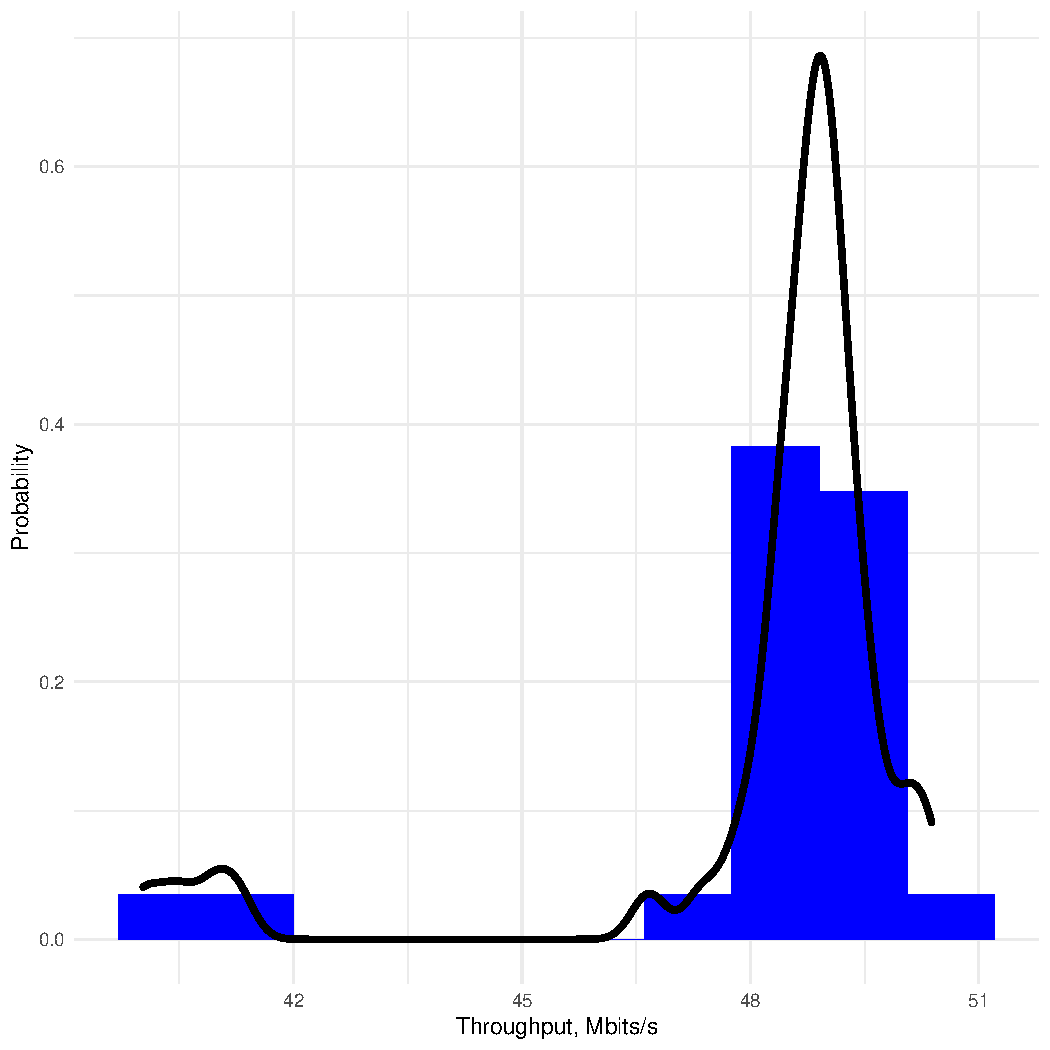
\includegraphics[width=0.9\textwidth]{graphics/throughput/download.pdf}
%    \caption{Download throughput, Mbit/s}
%    \label{fig:download}
%\end{figure}

%\begin{figure}[h!]
%    \centering
%    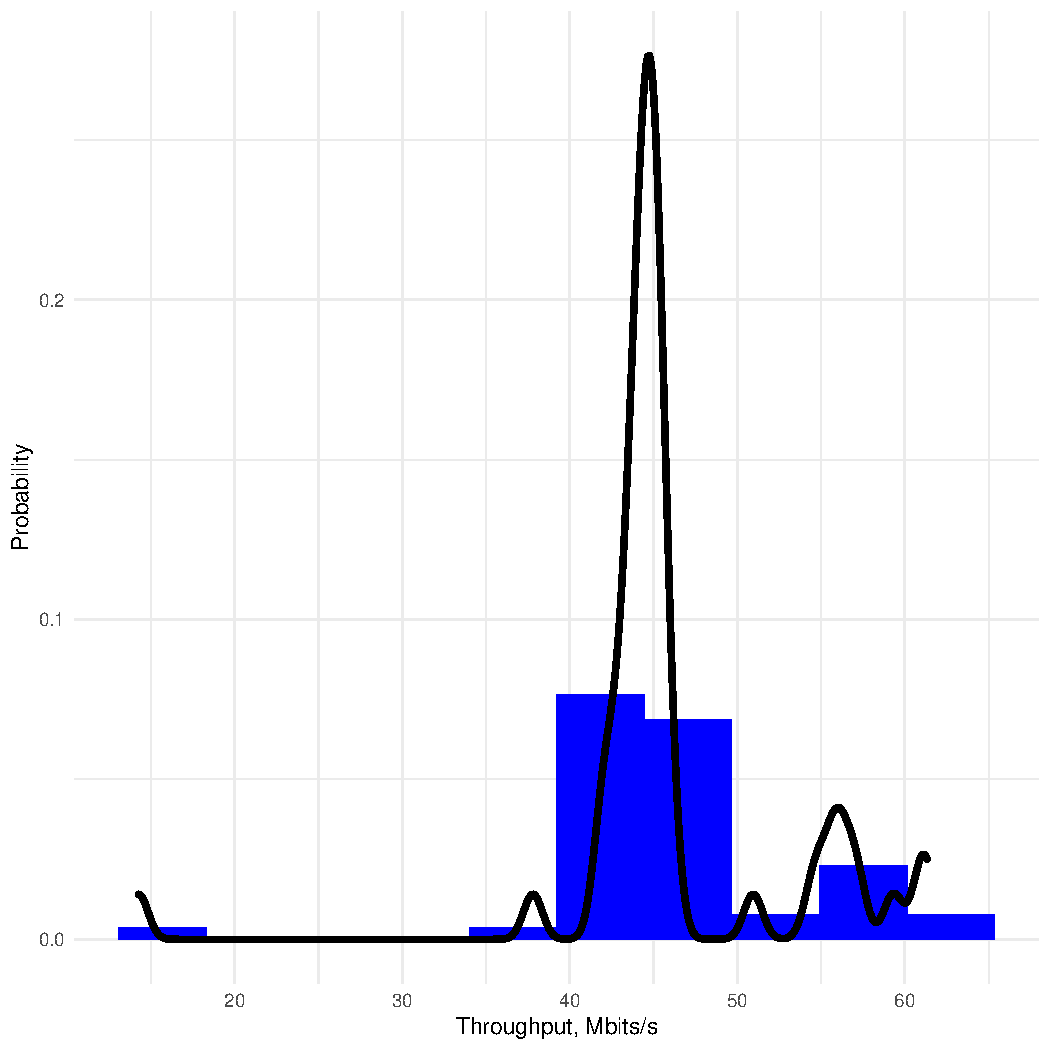
\includegraphics[width=0.9\textwidth]{graphics/throughput/upload.pdf}
%    \caption{Upload throughput, Mbit/s}
%    \label{fig:upload}
%\end{figure}

%\begin{figure}[h!]
%    \centering
%    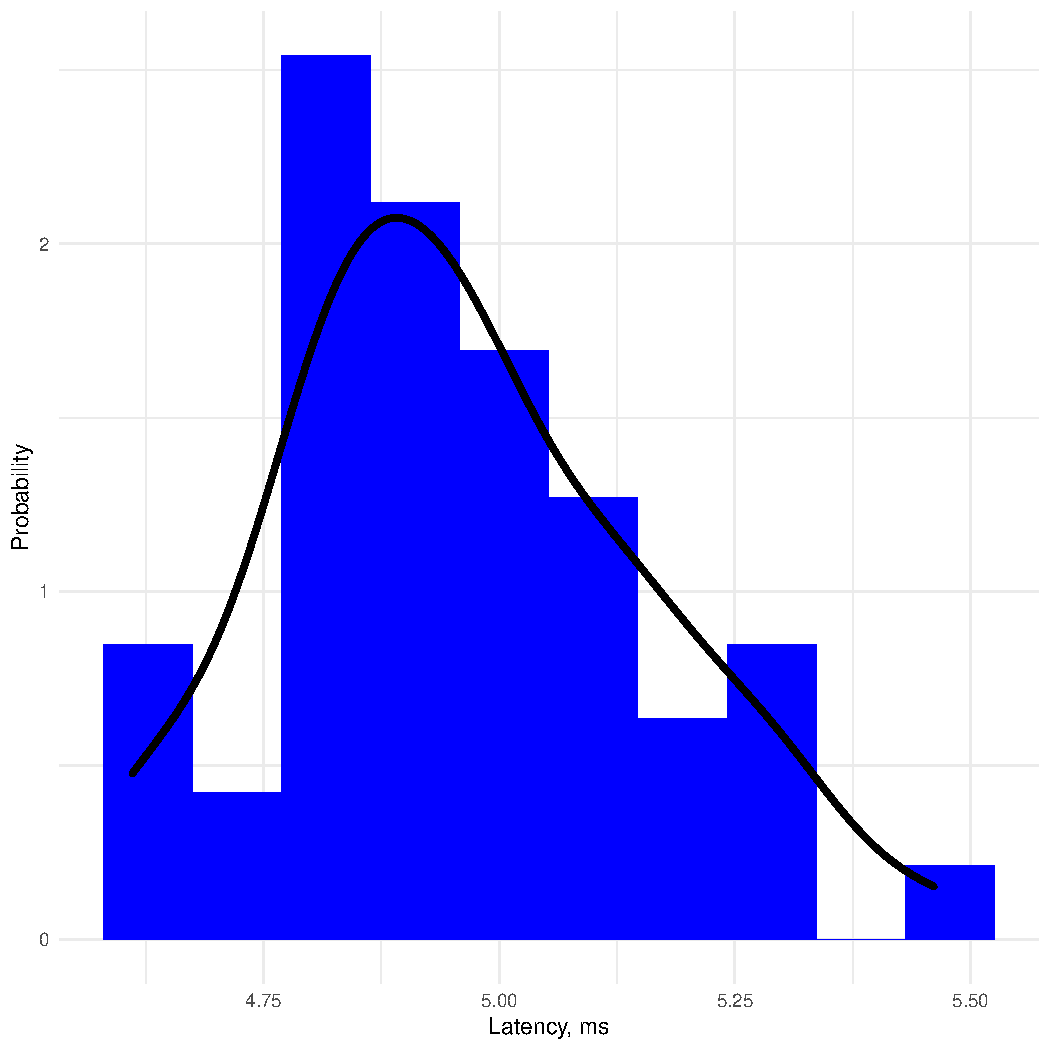
\includegraphics[width=0.9\textwidth]{graphics/throughput/ping.pdf}
%    \caption{Ping latency, ms}
%    \label{fig:ping}
%\end{figure}

\section{Scalable multipoint to multipoint VPN using HIP protocol}

The overall architecture which we have implemented in
Mininet framework is shown in Figure~\cite{fig:l3vpn}. The architecture
of the distributed L3-VPN network is of hub-and-spoke type.
Hub nodes comprise the backbone of the network, whereas,
multiple spoke PE elements are attached to the hubs. This
allows to achieve scalability property. The security of the 
network is achieved by using Host Identity Protocol to negotiated
the authentication and encryption keys, whereas, the actual packet authentication
and encryption is performed on hop-by-hop bases using HMAC-SHA256
algorithm. 

\begin{figure}[h!]
    \centering
    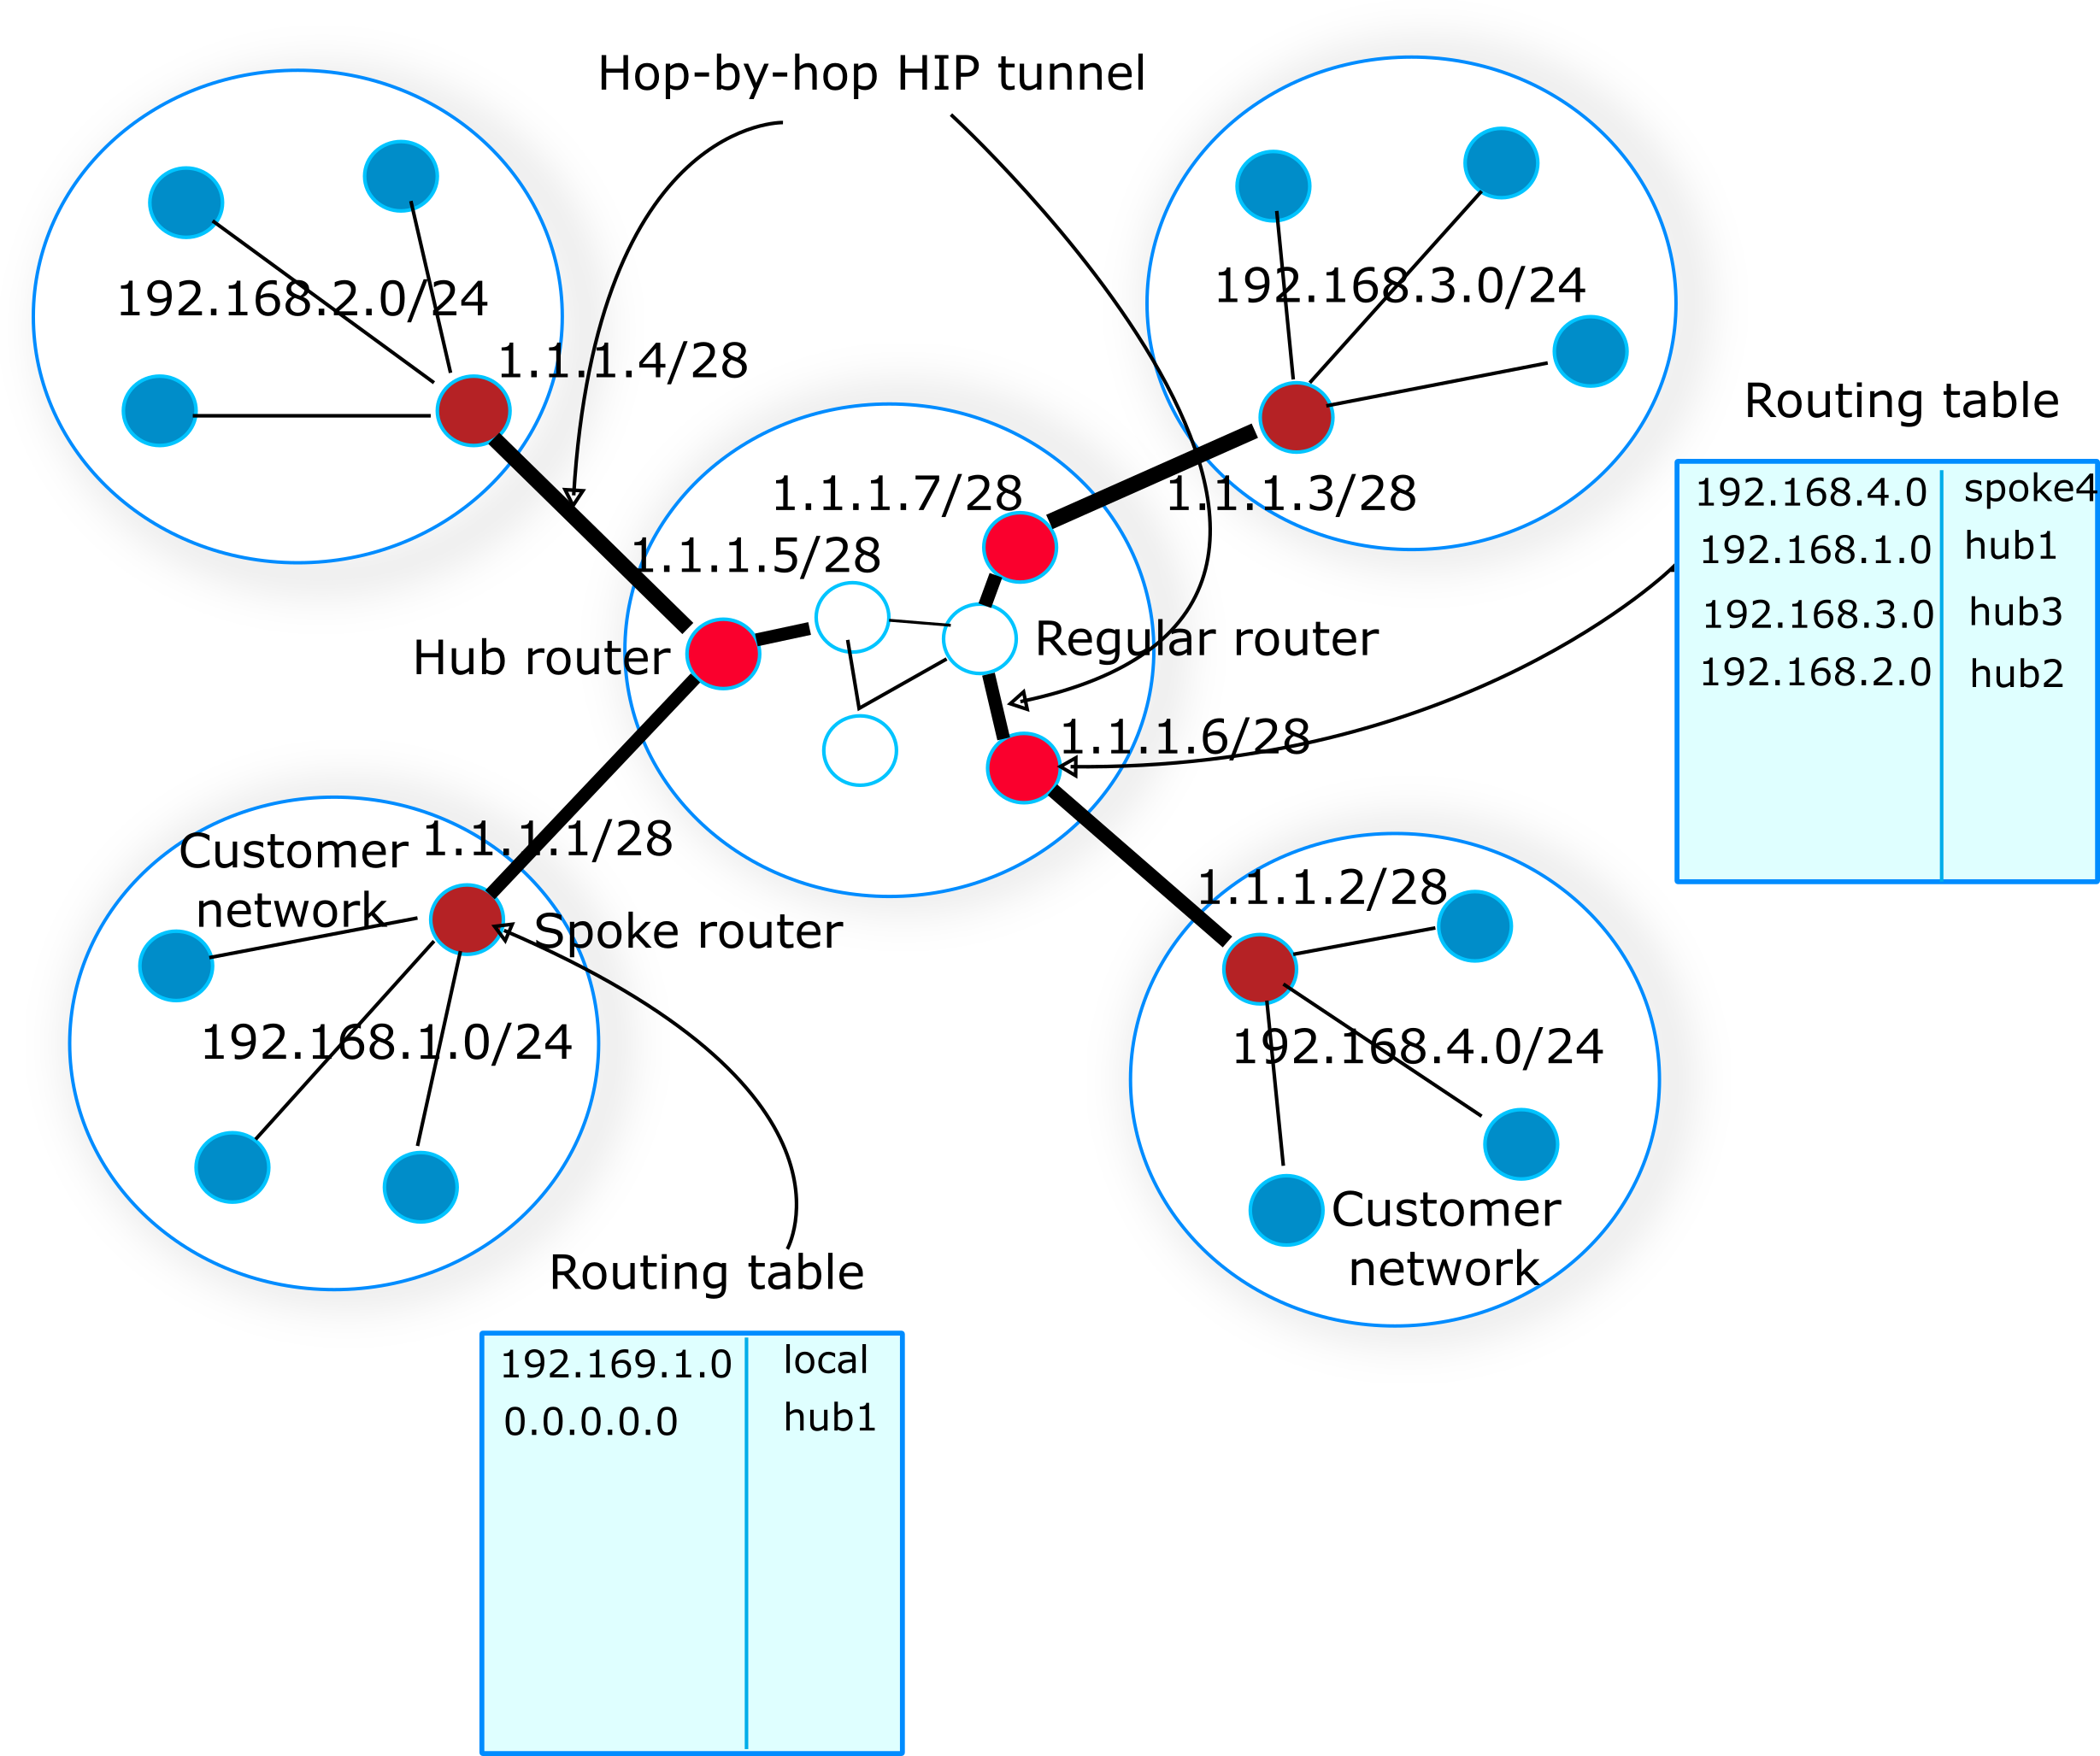
\includegraphics[width=0.9\textwidth]{graphics/l3-vpn.png}
    \caption{HIP-based L3-VPN in Mininet}
    \label{fig:l3vpn}
\end{figure}

\section{Comparison of various solutions}

In what follows, we compare now different approaches, identify there
characteristics and limitation. In Table~\cite{tab:analysis} we 
compare three different approaches for building overlays with Host 
Identity Protocol. 

\begin{table*}
    \small
    \begin{tabular}{|l|c|c|c|}
    \hline
    Characteristic $\downarrow$ \ Overlay type $\rightarrow$ & L2-VPN & L3-VPN & HIP-VPLS \\\hline
    Size of forwarding/routing table & $O(n)$ & $O(m)$ & $O(n)$\\\hline
    Number of links in mesh & $O(k^2)$ & $O(k^2)$ & $O(l^2)$ \\\hline
    Privacy (exposure of information) & MACs & IPs & No \\\hline
    Encryption and authentication & Hop-by-hop & Hop-by-hop & PE-to-PE \\\hline
    Tunneling mode & Ethernet-in-IP & IP-in-IP & Ethernet-in-IP \\\hline
    Loop free-topology & 802.1d & Controller & Not required \\\hline
    \end{tabular}
    \label{tab:analysis}
    \caption {Comparison study of different multipoint VPLS/VPN designs}
\end{table*}

\chapter{Conclusions}






